\section{Анализ методов машинного обучения для классификации признаков}

В настоящее время существует множество методов и алгоритмов компьютерного зрения, предложеных и развитых для классификации данных.

Особенности систем машинного зрения позволяют вырабатывать требования для разработки методов и алгоритмов классификации. Кроме того, тип данных является решающим фактором адекватности и точности классификации \cite{segi1998}, \cite{sophi2000}. Было много исследований в которых успешно применяются алгоритмы и методы компьютерного зрения для классификации данных, таких как распознавание жестов \cite{Phan2013}, распознавание лиц \cite{Phakhi2013, Goldstein1991}, идентификация деятельности человека \cite{Kang2006, Saaidi2008}. Адаптивные методы распознавания объектов и классификации основаны на автоматической подстройке к свойствам обрабатываемых данных, что позволяет разработать распознающую систему с приемлемыми характеристиками \cite{anwef2011}. Ко второй категории относятся методы, характеризующиеся сокращением размерности данных \cite{Belhumeur1997}, \cite{Hallinan1999}. Ниже изложим наиболее популярные методы классификации.

\subsection{Алгоритм AdaBoost}

Алгоритм AdaBoost был разработан Йоавом Фройндом (Yoav Freund) и Робертом Шапиром (Robert Schapire) в 1996 году \cite{Freund1997}, \cite{Freund1996}. Этот алгоритм <<адаптивность и усиление>> используется для создания классификатора. Как известно, классификатор на входе принимает набор данных для обучения и пытается предсказать или классифицировать новые образцы данных, которые относятся к определенному классу \cite{Sochman2004} (рис. \ref{img6}). Алгоритм AdaBoost построен на основе алгоритмов обучения (например, деревья решений) и объединения их. Цель состоит в том, чтобы создать один сильный классификатор на основе нескольких слабых классификаторов. Алгоритм AdaBoost успешен в поиске личной информации на статических изображениях \cite{Su2005}. Сайты постоянно поддерживают поиск информации на основе изображений используя AdaBoost.

Система поиска лица на основе алгоритма <<Viola-Jones>> \cite{Viola2001}, \cite{Violaj2001} также использует AdaBoost. Эти системы работают с высокой точностью, например в цифровых фотокамерах и смартфонах. Вейвлет Хаара \cite{Viola2004} являются одним из простых признаков, которые обычно используется на практике. Но размер такого вектора-признака довольно большой (162,336). Таким образом, нужно применять метод главных компонентов (англ. principal component analysis, PCA) \cite{Masoud2005} для увеличения или уменьшения размера и выбора новых функций. После этого полученные данные классифицируются алгоритмом AdaBoost.


\begin{figure}[ht!]
\centering
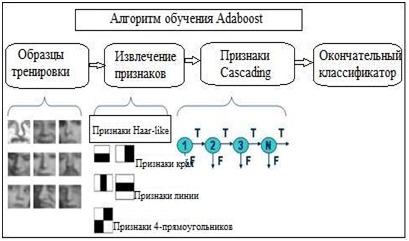
\includegraphics [scale=0.8] {images/h6.png}
\begin{center}
%\captionsetup{justification=justified, labelsep=period}
\caption{Описание алгоритма AdaBoost \cite{Sochman2004}.} \label{img6}
\end{center}
\end{figure}

Этот алгоритм прост и удобен а также, имеет очень высокую скорость обучения.  Алгоритм AdaBoost гибкий и универсальный, может быть объединен с любым алгоритмом машинного обучения, и может работать с большим количеством различных данных.

\subsection{Искусственные нейронные сети}

Нейронная сеть была успешно использована для решения задач классификации объекта \cite{Hinton2012}. С точки зрения машинного обучения, искусственные нейронные сети (ИНС) являются вычислительными моделями, которые способны решать задачи распознавания образов \cite{Sergios2006}, \cite{Dunne2007}. Нейронную сетевую архитектуру можно разделить на две основные группы: сети прямой связи \cite{Colin2000} и обратного распространения сети \cite{Kamruzzaman2006}. При решении задачи классификации возраста и пола человека применяется большое количество нейронных сетей различных архитектур \cite{Rowley1998}, в частности: вероятностные нейронные сети (probabilistic decision-based neural networks) \cite{Lin1997}, многослойные персептроны \cite{Juell1996} и т.д. Нейронные сеть - ИНС являются одним из приоритетных направлений исследований в области машинного обучения.

Действительно, искуственные нейронные сети способны решить различные проблемы: классификация образов, аппроксимации функций, оптимизация и квантование вектора пространства данных, в то время как традиционные методы не могут эффективно решить вышеуказанные проблемы.

\subsection{Метод опорных векторов}

Метод опорных векторов (Support Vector Machines, МОВ)  используется для решения задач классификации и регрессионного анализа. Этот метод был предложен В. Вапником и А. Червоненкисом в 1995 году \cite{Vapnik1995}. Особые свойства МОВ – это непрерывное уменьшение эмпирической ошибки классификации. Использование МОВ и мешка признаков (Bag-of-Features) оказалось эффективным в задачах обнаружения и распознавания жестов на видеопоследовательности \cite{Nasser2011, Dardas2010}, а также при решении других задач \cite{Jiang2007, Lazebnik2006}. Метод опорных векторов (МОВ) позволил классифицировать нормальные и ненормальные поведения человека \cite{Yogameena2010}. В работе \cite{Nguyen2015} авторы представили предлагаемый подход к классификации пола и размера одежды с помощью метода опорных векторов. Алгоритм работал с антропометрическими данными для классификации по двум классам: мужчины / женщины.

Метод опорных векторов, как и методы на основе деревьев решений даёт высокую точность для наборов данных с непрерывными типами данных (непрерывное значение). Они являются двумя методами, которые обычно используются для классификации данных. Тем не менее, не существует универсального метода классификации. Результат всегда зависит от цели системы и типов данных. Кроме того, выбор ядра и других параметров является  слабостю МОВ.

\subsection{Алгоритм случайного леса (Random Forest)}

Random Forest (случайный лес) \cite{Breiman2002, Breiman2001} является развитием семейства алгоритмов, разработанных Лео Брейман в университете Калифорнии, Беркли. На самом деле, Random Forest использует методы, называемые мешки (bagging). Эта методика позволяет выбрать подмножество атрибутов в каждом узле дерева классификатора, чтобы разделить его на следующий уровень. Таким образом, Random Forest имеет возможность разделить очень большое пространство поиска на меньшие пространства поиска. Таким образом, алгоритм может выполнять сортировки быстро и легко.

В случайном лесе, разработка набора деревьев значительно улучшила точность классификации, каждое дерево в наборе будет <<голосовать>> за самый популярный класс. Для развития наборов деревьев, как обычно, создаются случайные векторы. Такие векторы будут регулировать развитие каждого дерева в вышеупомянутом наборе. Для дерева $K$ в наборе, случайный вектор $\theta_k$  генерируется, независимый с генерированными векторами ранее $\theta_1, \theta_2, ..., \theta_{k-1}$, но распределение таких векторов одинаково. 

Дерево было разработано на основе обучающего множества и вектора $\theta_k$. Получается результат: подкласс $h\left(x, \theta_k \right)$ где $х$ - входной вектор. После создания большого количества деревьев, проводится голосование <<голосовать>> за самый популярный класс.

Случайный лес определяется следующим образом \cite{Biggio2011}: подкласс случайного леса, состоящий из наборов слоистой структуры дерева $\left\{h\left(x,\theta_k\right), k=1, ...,n\right\}$ где $\left\{\theta_k\right\}$- независимые векторы, также случайным образом распределенные, и каждое дерево даёт один голос для наиболее популярного класса в входном векторе $х$.

Основная идея алгоритма случайного леса:

\begin{itemize}
	\item В каждом подразделении деревьев, случайный набор m атрибутов взят из m таких атрибутов, которые участвуют в распределении деревьев;
	\item -	Первый шаг в оценке важности переменной в тренировочном наборе – тренировка случайного леса в этом наборе. Во время процесса построения модели для каждого элемента тренировочного набора считаются так называемой <<out-of-bag>> ошибкой. Затем для каждой сущности такая ошибка усредняется по всему случайному лесу.
\end{itemize}

По алгоритмам Random Forest (случайного леса) отметили, что случайный лес является хорошим методом классификации, потому что: 1) в методе Random Forest, ошибки были сведены к минимуму в результате случайного леса, синтезированию через обучения (learner), 2) случайный выбор на каждом этапе в Random Forest снизит корреляцию между учащимися в синтезе результатов. Кроме того, мы также обнаружили, что общая ошибка из слоистых лесных деревьев зависит от их индивидуальных ошибок в лесных деревьях, а также корреляции между деревьями.